%%%%%%%%%%%%%%%%%
% Configuration %
%%%%%%%%%%%%%%%%%

\documentclass[12pt, a4paper, twocolumn]{article}
\usepackage{amsmath}
\usepackage{amssymb}
\usepackage{mathtools}
\usepackage{csquotes}
\usepackage{xurl}
\usepackage{hyperref}
\hypersetup{colorlinks=true, urlcolor=blue, linkcolor=blue, citecolor=blue}
\urlstyle{rm}
\usepackage[super,comma,sort&compress]{natbib}
\bibliographystyle{plainnat}
\usepackage{abstract}
\renewcommand{\abstractnamefont}{\normalfont\bfseries}
\renewcommand{\abstracttextfont}{\normalfont\itshape}
\usepackage{lipsum}
\usepackage{booktabs}
\usepackage{geometry}
\geometry{top=1cm,bottom=1.5cm,left=2cm,right=2cm,includehead,includefoot}
\setlength{\columnsep}{7mm} % Column separation width
\renewcommand*{\thefootnote}{\roman{footnote}} % Use symbols for footnotes
\renewcommand*{\bibfont}{\raggedright}
\usepackage{float}
\usepackage{graphicx}
\usepackage{subcaption}
\usepackage{bm}

% Inline equations: https://tex.stackexchange.com/a/78582/178803
\makeatletter
\newcommand*{\inlineequation}[2][]{%
  \begingroup
    % Put \refstepcounter at the beginning, because
    % package `hyperref' sets the anchor here.
    \refstepcounter{equation}%
    \ifx\\#1\\%
    \else
      \label{#1}%
    \fi
    % prevent line breaks inside equation
    \relpenalty=10000 %
    \binoppenalty=10000 %
    \ensuremath{%
      % \displaystyle % larger fractions, ...
      #2%
    }%
    ~\@eqnnum
  \endgroup
}
\makeatother

%%%%%%%%%%%%%%
% References %
%%%%%%%%%%%%%%

\begin{filecontents}{value_based_prioritization.bib}

@InCollection{scientific-method,
  author       = {Andersen, Hanne and Hepburn, Brian},
  title        = {Scientific Method},
  booktitle    = {The Stanford Encyclopedia of Philosophy},
  editor       = {Edward N. Zalta},
  note         = {\url{https://plato.stanford.edu/archives/sum2016/entries/scientific-method/}},
  year         = {2016},
  edition      = {Summer 2016},
  publisher    = {Metaphysics Research Lab, Stanford University},
}

@article{martela2016three,
  title        = {The three meanings of meaning in life: Distinguishing coherence, purpose, and significance},
  author       = {Martela, Frank and Steger, Michael F},
  journal      = {The Journal of Positive Psychology},
  volume       = {11},
  number       = {5},
  pages        = {531--545},
  year         = {2016},
  publisher    = {Taylor \& Francis},
  note         = {\url{https://www.ippanetwork.org/wp-content/uploads/2017/02/Martela-Steger-JOPP.pdf}},
}

@book{huemer2007ethical,
  title        = {Ethical Intuitionism},
  author       = {Huemer, Michael},
  year         = {2007},
  publisher    = {Springer},
  note         = {\url{https://spot.colorado.edu/~huemer/5.htm}},
}

@book{huemer2013problem,
  title        = {The Problem of Political Authority},
  author       = {Huemer, Michael},
  year         = {2013},
  publisher    = {Springer},
  note         = {\url{https://spot.colorado.edu/~huemer/1.htm}},
}

@InCollection{value-theory,
  author       = {Schroeder, Mark},
  title        = {Value Theory},
  booktitle    = {The Stanford Encyclopedia of Philosophy},
  editor       = {Edward N. Zalta},
  note         = {\url{https://plato.stanford.edu/archives/fall2016/entries/value-theory/}},
  year         = {2016},
  edition      = {Fall 2016},
  publisher    = {Metaphysics Research Lab, Stanford University},
}

@InCollection{consequentialism,
  author       = {Sinnott-Armstrong, Walter},
  title        = {Consequentialism},
  booktitle    = {The Stanford Encyclopedia of Philosophy},
  editor       = {Edward N. Zalta},
  note         = {\url{https://plato.stanford.edu/archives/win2015/entries/consequentialism/}},
  year         = {2015},
  edition      = {Winter 2015},
  publisher    = {Metaphysics Research Lab, Stanford University},
}

@InCollection{ayn-rand,
  author       = {Badhwar, Neera K. and Long, Roderick T.},
  title        = {Ayn Rand},
  booktitle    = {The Stanford Encyclopedia of Philosophy},
  editor       = {Edward N. Zalta},
  note         = {\url{https://plato.stanford.edu/archives/fall2017/entries/ayn-rand/}},
  year         = {2017},
  edition      = {Fall 2017},
  publisher    = {Metaphysics Research Lab, Stanford University},
}

@InCollection{religion-morality,
  author       = {Hare, John},
  title        = {Religion and Morality},
  booktitle    = {The Stanford Encyclopedia of Philosophy},
  editor       = {Edward N. Zalta},
  note         = {\url{https://plato.stanford.edu/archives/win2014/entries/religion-morality/}},
  year         = {2014},
  edition      = {Winter 2014},
  publisher    = {Metaphysics Research Lab, Stanford University},
}

@InCollection{morality-biology,
  author       = {FitzPatrick, William},
  title        = {Morality and Evolutionary Biology},
  booktitle    = {The Stanford Encyclopedia of Philosophy},
  editor       = {Edward N. Zalta},
  note         = {\url{https://plato.stanford.edu/archives/spr2016/entries/morality-biology/}},
  year         = {2016},
  edition      = {Spring 2016},
  publisher    = {Metaphysics Research Lab, Stanford University},
}

@InCollection{epicurus,
  author       = {Konstan, David},
  title        = {Epicurus},
  booktitle    = {The Stanford Encyclopedia of Philosophy},
  editor       = {Edward N. Zalta},
  note         = {\url{https://plato.stanford.edu/archives/sum2018/entries/epicurus/}},
  year         = {2018},
  edition      = {Summer 2018},
  publisher    = {Metaphysics Research Lab, Stanford University},
}

@InCollection{stoicism,
  author       = {Baltzly, Dirk},
  title        = {Stoicism},
  booktitle    = {The Stanford Encyclopedia of Philosophy},
  editor       = {Edward N. Zalta},
  note         = {\url{https://plato.stanford.edu/archives/sum2018/entries/stoicism/}},
  year         = {2018},
  edition      = {Summer 2018},
  publisher    = {Metaphysics Research Lab, Stanford University},
}

@InCollection{rawls,
  author       = {Wenar, Leif},
  title        = {John Rawls},
  booktitle    = {The Stanford Encyclopedia of Philosophy},
  editor       = {Edward N. Zalta},
  note         = {\url{https://plato.stanford.edu/archives/spr2017/entries/rawls/}},
  year         = {2017},
  edition      = {Spring 2017},
  publisher    = {Metaphysics Research Lab, Stanford University},
}

@InCollection{communitarianism,
  author       = {Bell, Daniel},
  title        = {Communitarianism},
  booktitle    = {The Stanford Encyclopedia of Philosophy},
  editor       = {Edward N. Zalta},
  note         = {\url{https://plato.stanford.edu/archives/sum2016/entries/communitarianism/}},
  year         = {2016},
  edition      = {Summer 2016},
  publisher    = {Metaphysics Research Lab, Stanford University},
}

@article{weinstein2009qalys,
  title        = {QALYs: the basics},
  author       = {Weinstein, Milton C and Torrance, George and McGuire, Alistair},
  journal      = {Value in health},
  volume       = {12},
  pages        = {S5--S9},
  year         = {2009},
  publisher    = {Wiley Online Library},
  note         = {\url{https://onlinelibrary.wiley.com/doi/pdf/10.1111/j.1524-4733.2009.00515.x}},
}

@article{zucchini2000introduction,
  title        = {An introduction to model selection},
  author       = {Zucchini, Walter},
  journal      = {Journal of mathematical psychology},
  volume       = {44},
  number       = {1},
  pages        = {41--61},
  year         = {2000},
  publisher    = {Academic Press},
  note         = {\url{http://www.indiana.edu/~clcl/Q550/Papers/Zucchini_JMP_2000.pdf}},
}

@article{wit2012all,
  title        = {‘All models are wrong...’: an introduction to model uncertainty},
  author       = {Wit, Ernst and Heuvel, Edwin van den and Romeijn, Jan-Willem},
  journal      = {Statistica Neerlandica},
  volume       = {66},
  number       = {3},
  pages        = {217--236},
  year         = {2012},
  publisher    = {Wiley Online Library},
  note         = {\url{https://www.rug.nl/research/portal/files/13270992/2012StatistNeerlWit.pdf}},
}

@misc{centers2017underlying,
  title        = {\textit{Underlying Cause of Death 1999-2017 on CDC WONDER Online Database, released December, 2018. Data are from the Multiple Cause of Death Files, 1999-2017, as compiled from data provided by the 57 vital statistics jurisdictions through the Vital Statistics Cooperative Program}},
  author       = {{Centers for Disease Control and Prevention and National Center for Health Statistics}},
  howpublished = {\url{https://wonder.cdc.gov/ucd-icd10.html}},
  note         = {Accessed: 2019-01-31},
}

@book{icd10,
  title        = {International statistical classification of diseases and related health problems},
  author       = {World Health Organization},
  year         = {2016},
  publisher    = {World Health Organization},
  edition      = {10th},
  note         = {\url{https://apps.who.int/iris/bitstream/handle/10665/246208/9789241549165-V1-eng.pdf}},
}

@article{anderson2004model,
  title        = {Model selection and multi-model inference},
  author       = {Anderson, DR and Burnham, K},
  journal      = {Second. NY: Springer-Verlag},
  year         = {2004},
}

@article{burnham2004multimodel,
  title        = {Multimodel inference: understanding AIC and BIC in model selection},
  author       = {Burnham, Kenneth P and Anderson, David R},
  journal      = {Sociological methods \& research},
  volume       = {33},
  number       = {2},
  pages        = {261--304},
  year         = {2004},
  publisher    = {Sage Publications Sage CA: Thousand Oaks, CA},
  doi          = {10.1177/0049124104268644},
  note         = {\url{http://www.sortie-nd.org/lme/Statistical\%20Papers/Burnham_and_Anderson_2004_Multimodel_Inference.pdf}},
}

@book{berk2004regression,
  title        = {Regression analysis: A constructive critique},
  author       = {Berk, Richard A},
  volume       = {11},
  year         = {2004},
  publisher    = {Sage},
}

@book{hyndman2018forecasting,
  title        = {Forecasting: principles and practice},
  author       = {Hyndman, Rob J and Athanasopoulos, George},
  year         = {2018},
  publisher    = {OTexts},
  note         = {\url{https://otexts.com/fpp2/}},
}

@article{clemen1989combining,
  title        = {Combining forecasts: A review and annotated bibliography},
  author       = {Clemen, Robert T},
  journal      = {International journal of forecasting},
  volume       = {5},
  number       = {4},
  pages        = {559--583},
  year         = {1989},
  publisher    = {Elsevier},
  note         = {\url{https://faculty.fuqua.duke.edu/\~clemen/bio/Published\%20Papers/13.CombiningReview-Clemen-IJOF-89.pdf}},
}

@article{taylor2018forecasting,
  title        = {Forecasting at scale},
  author       = {Taylor, Sean J and Letham, Benjamin},
  journal      = {The American Statistician},
  volume       = {72},
  number       = {1},
  pages        = {37--45},
  year         = {2018},
  publisher    = {Taylor \& Francis},
  note         = {\url{https://peerj.com/preprints/3190.pdf}},
}

@article{makridakis2018m4,
  title        = {The M4 Competition: Results, findings, conclusion and way forward},
  author       = {Makridakis, Spyros and Spiliotis, Evangelos and Assimakopoulos, Vassilios},
  journal      = {International Journal of Forecasting},
  volume       = {34},
  number       = {4},
  pages        = {802--808},
  year         = {2018},
  publisher    = {Elsevier},
  note         = {\url{https://www.researchgate.net/profile/Spyros_Makridakis/publication/325901666_The_M4_Competition_Results_findings_conclusion_and_way_forward/links/5b2c9aa4aca2720785d66b5e/The-M4-Competition-Results-findings-conclusion-and-way-forward.pdf}},
}

@misc{censusestimates19001999,
  title        = {\textit{Historical National Population Estimates}},
  author       = {{U.S. Census Bureau}},
  howpublished = {\url{https://www2.census.gov/programs-surveys/popest/tables/1900-1980/national/totals/popclockest.txt}},
  note         = {Accessed: 2019-02-23},
}

@misc{worldbankopendata,
  title        = {\textit{World Bank Open Data: United States SP.POP.TOTL}},
  author       = {{World Bank}},
  howpublished = {\url{http://api.worldbank.org/v2/en/country/USA?downloadformat=csv}},
  note         = {Accessed: 2019-02-23},
}

@misc{nbermortality,
  title        = {\textit{Mortality Data: Vital Statistics NCHS' Multiple Cause of Death Data, 1959-2017}},
  author       = {{The National Bureau of Economic Research}},
  howpublished = {\url{https://www.nber.org/data/vital-statistics-mortality-data-multiple-cause-of-death.html}},
  note         = {Accessed: 2019-02-23},
}

@misc{icdcomparabilityratios,
  title        = {{A Guide to State Implementation of ICD-10 for Mortality; Part II: Applying Comparability Ratios}},
  author       = {{Centers for Disease Control and Prevention and National Center for Health Statistics}},
  howpublished = {\url{https://www.cdc.gov/nchs/data/statab/document-for-the-states.pdf}},
  note         = {Accessed: 2019-02-23},
}

\end{filecontents}

\begin{document}

\title{Value-Based Prioritization\thanks{\url{https://github.com/freeradical13/ValueBasedPrioritization}}}

\author{Kevin Grigorenko\thanks{\href{mailto:kevin@myplaceonline.com}{kevin@myplaceonline.com}}}

\newcommand{\abstractText}{\noindent
A method is proposed to use value theory to quantitatively prioritize
potential actions to accomplish a goal. This method is applied to the
example of choosing meaningful work using an example value system based
on the desire to reduce suffering.
}

%%%%%%%%%%%%
% Abstract %
%%%%%%%%%%%%

\twocolumn[
  \begin{@twocolumnfalse}
    \maketitle
    \begin{abstract}
      \abstractText
      \newline
      \newline
    \end{abstract}
  \end{@twocolumnfalse}
]

\saythanks

%%%%%%%%%%%
% Article %
%%%%%%%%%%%

\section{Introduction}

Why should a particular goal be pursued (\enquote{Why})? Given a goal, what actions should be pursued to best accomplish said goal (\enquote{What})? Given an action, how should said action be pursued (\enquote{How})?

This article proposes that value theory usually best scopes \enquote{Why} and \enquote{What} and the scientific method usually best answers \enquote{How}. A method called Value-Based Prioritization is developed to answer the \enquote{What} question:

\begin{equation*}
  \begin{gathered}
    \textrm{Why: } \textit{Value Theory} \\
    \downarrow \\
    \textrm{What: } \textit{\textbf{Value-Based Prioritization}} \\
    \downarrow \\
    \textrm{How: } \textit{Scientific Method}
  \end{gathered}
\end{equation*}

\section{Why a Goal?}

\enquote{Why a Goal?} is usually best scoped using value systems because they are evaluative by nature\cite{value-theory}. Evaluating different value systems is left as an (lifelong) exercise for the reader\footnote{Example value systems include intuitionism\cite{huemer2007ethical}, consequentialism\cite{consequentialism}, evolutionary biology\cite{morality-biology}, religion\cite{religion-morality}, epicureanism\cite{epicurus}, stoicism\cite{stoicism}, political liberalism\cite{rawls}, anarcho-capitalism\cite{huemer2013problem}, communitarianism\cite{communitarianism}, objectivism\cite{ayn-rand}, etc.}.

\section{What Actions?}

\enquote{What Actions?} is usually best scoped by prioritizing actions because actions usually have differing effect sizes and time is limited. It follows from the value system used to answer \enquote{Why} that the same value system is used primarily to evaluate the priority of each action.

This article proposes a method called Value-Based Prioritization which builds a quantitative prioritization model based on predicted effect sizes. Raw prioritization scores are further scaled by contextual factors such as implementation time, cost, risk, and other judgments.

\section{How to do an Action?}

Given answers to \enquote{Why?} and \enquote{What?}, how to implement actions is usually best answered with the scientific method\cite{scientific-method}: observations are made and rational thought is used to generate hypotheses, hypotheses are tested with experiments, and successful experiments lead to theories and results.

\section{Value-Based Prioritization}

A \textbf{value system} \inlineequation[value-system]{V} generates a \textbf{goal} \inlineequation[goal]{G(t)} (for some future time $t$) and a set of \textbf{mutually exclusive potential future actions} $A(t)$:

\begin{equation}\label{potential-actions}
  \begin{gathered}
    A(t) = \{A_1(t), \ldots, A_N(t)\}, \\
    N > 1
  \end{gathered}
\end{equation}

An action's \textbf{estimated relative accomplishment amount} $B(A(t))$ is an action's expected \textit{relative} (i.e. with respect to other actions) contribution towards accomplishing $G$(t):

\begin{equation}\label{action-amount}
  \begin{gathered}
    B(A(t)) = \mathbb{R}, \\
    0 \leq \mathbb{R} \leq 1
  \end{gathered}
\end{equation}

Thus, $G(t)$ is fully accomplished if all actions are accomplished:

\begin{equation}\label{goal-accomplished}
  G(t) = \sum_{i=1}^{N} B(A_i(t)) = 1
\end{equation}

A \textbf{value-based prioritization score} $C(A(t))$ is the result of the product of a set of \textbf{value-based prioritization scale functions} \inlineequation[scale-functions]{S = \{S_1, \ldots, S_N\}} multiplied by \eqref{action-amount}:

\begin{equation}\label{prioritization-score}
  \begin{gathered}
    C(A(t)) = B(A(t)) \cdot \prod_{j=1}^{N} S_j(A(t)), \\
    0 \leq S_j(B(A(t))) \leq 1
  \end{gathered}
\end{equation}

Example scale functions include implementation time, cost, risk, and other judgments. Ideally, scale functions should be defined before running the model to reduce bias. The set $S$ always includes the element $S_1(A(t)) = 1$. Note that $\sum_{i=1}^{N} C(A_i(t)) \neq G$ if any $S_j(A_i(t)) < 1$.

A \textbf{value-based prioritization} $Z(t)$ is a sequence of actions ordered by prioritization score \eqref{prioritization-score} in descending order:

\begin{equation}\label{vbp}
  \begin{gathered}
    Z(t) = (A_1(t), \ldots, A_N(t)), \\
    C(A_1(t)) \geq \ldots \geq C(A_N(t))
  \end{gathered}
\end{equation}

The first $k$ actions in $Z(t)$ should be executed in descending priority/proportion where \inlineequation[how-many-actions]{k} is chosen based on factors such as available concurrency, time, resources, etc.

\section{Modeled Value-Based Prioritization}

Historical data may be used to predict actions' estimated relative accomplishment amounts \eqref{action-amount} at a future time \inlineequation[modeled-future-time]{t_F} (e.g. the average time actions will take to ramp up implementation).

If each action has historical data $D(A)$:

\begin{equation}\label{action-predictors}
  \begin{multlined}
    D(A) = \\
    \shoveleft[0.5cm]{((t_1, D(A,t_1)), \ldots, (t_N, D(A,t_N)))}
  \end{multlined}
\end{equation}

Then, a set of \textbf{comparable prediction models} $R(D(A))$ is applied to each $D(A)$ (e.g. exponential smoothing\cite{hyndman2018forecasting}\textsuperscript{,}\footnote{\scriptsize{\url{https://otexts.com/fpp2/expsmooth.html}}}, ARIMA\cite{hyndman2018forecasting}\textsuperscript{,}\footnote{\scriptsize{\url{https://otexts.com/fpp2/arima.html}}}, linear regression\cite{hyndman2018forecasting}\textsuperscript{,}\footnote{\scriptsize{\url{https://otexts.com/fpp2/regression.html}}}, machine learning\cite{makridakis2018m4}, seasonal algorithms such as TBATS\cite{hyndman2018forecasting}\textsuperscript{,}\footnote{\scriptsize{\url{https://otexts.com/fpp2/advanced.html}}}, etc.):

\begin{equation}\label{prediction-models}
  \begin{multlined}
    R(D(A)) =\\
    \{R_1(D(A)), \ldots, R_N(D(A))\}
  \end{multlined}
\end{equation}

The models are compared using \textbf{model selection} (or forecasting)\cite{hyndman2018forecasting,taylor2018forecasting,wit2012all,zucchini2000introduction}\textsuperscript{,}\footnote{\scriptsize{\url{https://otexts.com/fpp2/selecting-predictors.html}}} using a model selection algorithm \inlineequation[model-selection]{L(R(D(A)))} (e.g. smallest Akaike's Information Criterion [AIC], smallest Corrected AIC [AICc], smallest Bayesian Information Criterion [BIC], smallest cross-validation, largest adjusted coefficient of determination [$\bar{R^2}$], etc.).

For each action, $L(R(D(A)))$ produces the \textbf{best fitting model} $M(A(t))$ (or a model that's an average of multiple models\cite{clemen1989combining}\textsuperscript{,}\footnote{\scriptsize{\url{https://otexts.com/fpp2/combinations.html}}}).

Each action's $M(A(t_F))$ is used to predict $B(A(t_F))$.

Finally, \textbf{modeled value-based prioritization} \inlineequation[modeled-vbp]{Z(t_F)} is simply \eqref{vbp} with $t_F$.

\section{Choosing Meaningful Work}

The following example applies modeled value-based prioritization \eqref{modeled-vbp} to the goal of choosing meaningful work\cite{martela2016three}. Every aspect is an example and should be reconsidered.

First, outline the parameters:

\begin{itemize}
  \item \eqref{value-system} $V = $ a value system which answers \enquote{Why work?} with \enquote{To reduce suffering} which is defined as maximal human suffering: death\footnote{More accurately, something like the lack of a potential of life.}. Alternatives include morbidity and disease burden (e.g. Quality-Adjusted Life Years [QALYs]\cite{weinstein2009qalys}), non-human suffering, pre-birth suffering, etc.
  \item \eqref{goal} $G(t) = $ eliminate human death.
  \item \eqref{potential-actions} $A(t) = $ the set of actions which would eliminate human death.
  \item \eqref{how-many-actions} $k = $ 1 for a single person (use 2 to hedge the failure of the first action or as a volunteer activity).
  \item \eqref{modeled-future-time} $t_F = $ 10 years; an average amount of time under normal conditions to integrate into a new career to work on some subset of $A(t)$ (including learning, certification, building experience, networking, etc.).
  \item \eqref{action-predictors} $D(A) = $ time-series data on human death by underlying cause\footnote{\url{https://www.who.int/topics/mortality/en/}}.
  \item \eqref{prediction-models} $R(D(A)) = $ exponential smoothing functions using Holt's linear trend method\footnote{\url{https://otexts.com/fpp2/holt.html}}\textsuperscript{,}\footnote{\url{https://otexts.com/fpp2/ets.html}}\textsuperscript{,}\footnote{\url{https://www.statsmodels.org/dev/examples/notebooks/generated/exponential_smoothing.html}}:
    \begin{equation*}
      \begin{gathered}
        \{ETS(A,A,N),ETS(A,A_d,N),\\
        ETS(A,M,N),ETS(A,M_d,N)\},\\
        \phi=0.98
      \end{gathered}
    \end{equation*}
  \item \eqref{model-selection} $L(R(D(A))) = $ lowest AICc.
\end{itemize}

$A(t)$ is the set of 179 actions which would eliminate the 179 major groups (ICD-10 sub-chapters\cite{icd10}) of underlying causes of death in the United States\cite{centers2017underlying,censusestimates19001999,worldbankopendata,nbermortality}\textsuperscript{,}\footnote{Group Results By \enquote{Year} And By \enquote{ICD Sub-Chapter}; Check \enquote{Export Results}; Uncheck \enquote{Show Totals}}\textsuperscript{,}\footnote{\texttt{python3 -m vbp.run count\char`_actions UnderlyingCausesOfDeathUnitedStates}}:

\begin{equation*}
  \begin{gathered}
    A(t) = \{\\
    A_1(t) = \textrm{Eliminate: Malignant neoplasms},\\
    A_2(t) = \textrm{Eliminate: Ischaemic heart diseases},\\
    \textrm{\ldots}\\
    A_{179}(t) = \textrm{Eliminate: Other disorders of ear}\\
    \}
  \end{gathered}
\end{equation*}

Review the list of actions\footnote{\texttt{python3 -m vbp.run list\char`_actions UnderlyingCausesOfDeathUnitedStates}} and hypothesize scale functions. Examples:

\begin{itemize}
  \item $S_1(A_i) = 1$
                  \newline\newline
                  Required scale function.
  \item $S_2(A_i) = \left(1 - \frac{AverageAge(A_i)}{MaxAge(A(t))}\right)$
                  \newline\newline
                  Scale towards younger people as they have more to lose.
  \item $S_3(A_i) = \left(\frac{(f(A_i)-min(f(A(t)))) \cdot (b-a)}{max(f(A(t))-min(f(A(t))}\right) + a$
                  \newline\newline
                  $f(A_i) = M'(A_i(t_F)), a=0.5, b=1$
                  \newline\newline
                  Scale down by up to half by the relative rate of change of an action's predicted rate of death: Take the derivative of $M(A_i(t))$ and evaluate it with the predicted value and min-max normalize\footnote{\scriptsize{\url{https://en.wikipedia.org/wiki/Normalization_(statistics)}}} into $[0.5,1]$ relative to other actions.
  \item $S_4(A_i) = \begin{cases}\text{0.1} & \mbox{if political/cultural} \\ \text{1} & \mbox{otherwise} \\ \end{cases}$
                  \newline\newline
                  Essentially remove actions that are primarily political and/or cultural.
\end{itemize}

The list does not include common scale functions such as implementation time, cost, risk, playing into strengths, piquing interest, market demand, return on investment, ramp-up time, interest, etc. because all medical actions are predicted to be in the same order of magnitude for those scales and all other actions are primarily political so they have a low score, rendering those scales moot.

Create a table listing all actions as rows and all \textit{manually calculated} scale functions as columns\footnote{For the example scale functions, this is only $S_4(A_i)$.}\textsuperscript{,}\footnote{\texttt{python3 -m vbp.run manual\char`_scale\char`_functions -t excel -o manual\char`_scale\char`_functions.xslx -n "Scale Values" -p "Eliminate: " UnderlyingCausesOfDeathUnitedStates S4}}:

\begin{table}[H]
  \centering
  \begin{tabular}{cccc}
    \toprule
      Action & $S_1$  & \ldots & $S_N$  \\
    \midrule
      $A_1$  & 0.1    &        & 1      \\
      $A_2$  & 1      &        & 0.25   \\
      \ldots &        &        &        \\
      $A_N$  & 0.99   &        & 0.9    \\
    \bottomrule
  \end{tabular}
  \caption{Theoretical scale function table}
  \label{table:scaletable}
\end{table}

For example:

\begin{table}[H]
  \centering
  \begin{tabular}{lc}
    \toprule
      Action                               & $S_4$ \\
    \midrule
      Eliminate: Assault                   & 0.1   \\
      Eliminate: Legal intervention \ldots & 0.1   \\
      Eliminate: Malnutrition              & 0.1   \\
      Eliminate: Transport accidents       & 0.1   \\
    \bottomrule
  \end{tabular}
  \caption{Example scale function table}
  \label{table:exscaletable}
\end{table}

Outside of the manually calculated scale function table, use obfuscated action names when developing the model to avoid introducing bias.

$D(A)$ for each action is the time-series data of number of deaths per year per 100,000 of population (\enquote{Crude Rate})\footnote{\url{https://wonder.cdc.gov/wonder/help/cmf.html\#Frequently\%20Asked\%20Questions\%20about\%20Death\%20Rates}}. For example, for \textit{Malignant neoplasms}\footnote{\texttt{python3 -m vbp.run action\char`_data UnderlyingCausesOfDeathUnitedStates "Malignant neoplasms"}}:

\begin{table}[H]
  \centering
  \begin{tabular}{cc}
    \toprule
      Year   & Crude Rate \\
    \midrule
      1999   &      197.0 \\
      \ldots &     \ldots \\
      2017   &      183.9 \\
    \bottomrule
  \end{tabular}
  \caption{Crude rate of deaths per year for \textit{Malignant neoplasms}}
  \label{table:daa1}
\end{table}

Run each comparable prediction model $R_i(D(A))$. For example, for \textit{Malignant neoplasms}\footnote{\texttt{python3 -m vbp.run predict UnderlyingCausesOfDeathUnitedStates --do-not-obfuscate -p 10 "Malignant neoplasms"}}:

\begin{figure}[H]
  \centering
  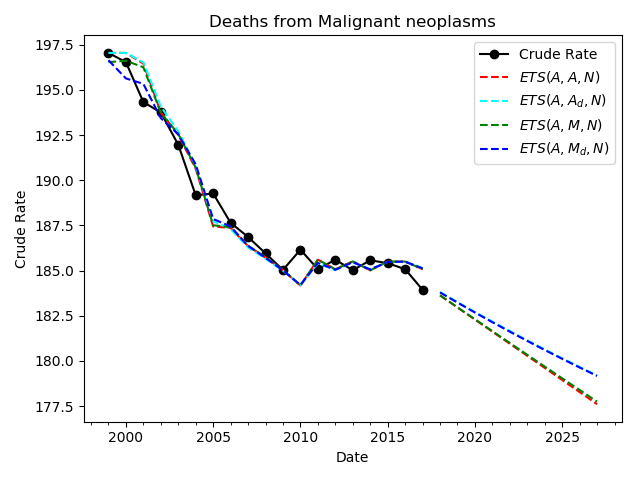
\includegraphics[width=0.5\textwidth]{Malignant_neoplasms_ets.png}
  \caption{Exponential smoothing functions $ETS(A,*,N),\phi=0.98$ using Holt's linear trend method for \textit{Malignant neoplasms}}\label{fig:neoplasmregs}
\end{figure}

Scedasticity, forecast uncertainty, and outliers are not considered because it's not clear how to automate processing of such data to tune or choose models.

For each model, calculate AICc and choose the model $M(A(t_F))$ that has the lowest AICc. For example:

\begin{table}[H]
  \centering
  \begin{tabular}{lcc}
    \toprule
      $R_i(D(A))$       & AICc           & Predicted       \\
    \midrule
      $ETS(A,A,N)$      & 13.43          & 177.60          \\
      $ETS(A,A_d,N)$    & 18.78          & 179.19          \\
      $\bm{ETS(A,M,N)}$ & \textbf{12.44} & \textbf{177.75} \\
      $ETS(A,M_d,N)$    & 14.35          & 179.17          \\
    \bottomrule
  \end{tabular}
  \caption{Example AICc values of $R_i(D(A))$ for \textit{Malignant neoplasms}}
  \label{table:choosem}
\end{table}

Use each $M(A(t_F))$ to calculate the predicted value and then generate all of the relative $B(t_F)$ values (setting negative values to 0) and any scale functions based on the models (e.g. scaling by the relative prediction derivatives using $S_3$). For example:

\begin{table}[H]
  \centering
  \begin{tabular}{lccc}
    \toprule
      Action  & $B(t_F)$ & $S_1$  & $S_3$  \\
    \midrule
      Action1 & 0.17     & 1.0    & 0.57   \\
      Action2 & 0.09     & 1.0    & 1      \\
      \ldots  & \ldots   & \ldots & \ldots \\
    \bottomrule
  \end{tabular}
  \caption{Example $B(t_F)$ values and model-based scale function values}
  \label{table:btable}
\end{table}

Combine the table above with the manually calculated scale functions table \ref{table:scaletable}. For example:

\begin{table}[H]
  \centering
  \begin{tabular}{lcccc}
    \toprule
      Action  & $B(t_F)$ & $S_1$  & $S_3$  & $S_4$  \\
    \midrule
      Action1 & 0.17     & 1.0    & 0.57   & 1      \\
      Action2 & 0.09     & 1.0    & 1      & 1      \\
      \ldots  & \ldots   & \ldots & \ldots & \ldots \\
    \bottomrule
  \end{tabular}
  \caption{Example $B(t_F)$ values, model-based scale function values, and manually calculated scale function values}
  \label{table:btablewithmanual}
\end{table}

Calculate any non-manually calculated and non-model based scale functions for each action\footnote{For the example scale functions, this is only $S_2(A_i)$} and create the final table with all scale functions. For example:

\begin{table}[H]
  \centering
  \begin{tabular}{lccccc}
    \toprule
      Action  & $B(t_F)$ & $S_1$  & $S_2$  & $S_3$  & $S_4$  \\
    \midrule
      Action1 & 0.17     & 1.0    & 1.0    & 0.57   & 1      \\
      Action2 & 0.09     & 1.0    & 1.0    & 1      & 1      \\
      \ldots  & \ldots   & \ldots & \ldots & \ldots \\
    \bottomrule
  \end{tabular}
  \caption{Example $B(t_F)$ values with all scale function values}
  \label{table:btablewithall}
\end{table}

Calculate the product of each action's $B(t_F)$ and its scale function values to produce the final $Z(t_F)$ table, then sort by the values in descending order and choose the top $k$ actions.

For the parameters and data in this example, the result is:

\begin{table}[H]
  \centering
  \begin{tabular}{clc}
    \toprule
      $k$ & Action          & $Z(t_F)$ \\
    \midrule
      1   & Eliminate: TODO & 0.08     \\
    \bottomrule
  \end{tabular}
  \caption{Example $Z(t_F)$ table}
  \label{table:ztable}
\end{table}

\section{Discussion}

The example modeling methods are crude and the field is ripe for more detailed approaches.

%%%%%%%%%%%%%%
% References %
%%%%%%%%%%%%%%

\bibliography{value_based_prioritization}

\end{document}

% Create PDF on Linux:
% FILE=value_based_prioritization; pkill -9 -f ${FILE} &>/dev/null; rm -f ${FILE}*aux ${FILE}*bbl ${FILE}*bib ${FILE}*blg ${FILE}*log ${FILE}*out ${FILE}*pdf &>/dev/null; pdflatex -halt-on-error ${FILE}; bibtex ${FILE} && pdflatex ${FILE} && pdflatex ${FILE} && (xdg-open ${FILE}.pdf &)
